% Intended LaTeX compiler: pdflatex
\documentclass[10pt,a4paper,UTF8]{article}
\usepackage{zclorg}
\usepackage{tikztheorem}
\author{张朝龙}
\date{}
\title{练习:正交补和极小化问题}
\hypersetup{
 pdfauthor={张朝龙},
 pdftitle={练习:正交补和极小化问题},
 pdfkeywords={},
 pdfsubject={},
 pdfcreator={Emacs 25.0.50.1 (Org mode 9.0.6)},
 pdflang={English}}
\begin{document}

\maketitle
\tableofcontents
\titlepic{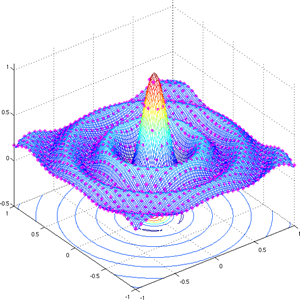
\includegraphics[scale=0.25]{../../img/sinc.PNG}}

\section{6.C.1}
\label{sec:org77828fb}


\begin{tikzproblem}
设\(v_{1},\ldots ,v_{m}\in V\),证明\(\{v_{1},\ldots ,v_{m}\}^{\bot}=  (\mathrm{span}(v_{1},\ldots ,v_{m}))^{\bot}\)
\end{tikzproblem}

\begin{tikzproof}
这个证明依赖于\(\langle v,u \rangle  =0\),则显然\(\langle \lambda v,u \rangle  = 0\)
\end{tikzproof}

\section{6.C.2}
\label{sec:orgff48754}


\begin{tikzproblem}
设\(U\)是\(V\)的有限维子空间,证明\(U^{\bot} = \{0\}\),当且仅当\(U=V\)
\end{tikzproblem}
\begin{tikzanswer}
显然,当\(U=V\)时,\(U^{\bot} = \{0\}\)。

另一方面,当\(U^{\bot} = \{0\}\),又因为\(V = U\oplus U^{\bot}\),所以\(U=V\)
\end{tikzanswer}

\section{6.C.3}
\label{sec:orgd3b714a}


\begin{tikzproblem}
设\(U\)是\(V\)的子空间,设\(u_{1},\ldots ,u_{m}\)是\(U\)的基,且\(u_{1},\ldots ,u_{m},w_{1},\ldots ,w_{n}\)是\(V\)的基。证明若对\(V\)的上述基应用格拉姆施密特过程得到组\(e_{1},\ldots ,e_{m},f_{1},\ldots ,f_{n}\),则\(e_{1},\ldots ,e_{m}\)是\(U\)的规范正交基,\(f_{1},\ldots ,f_{n}\)是\(U^{\bot}\)的规范正交基。
\end{tikzproblem}

\begin{tikzanswer}
格拉姆施密特过程:
设\(v_{1},\ldots ,v_{m}\)是\(V\)中线性无关组,设\(e_{1} = v_{1}/ \| v_{1} \|\),对于\(j=2,\ldots ,m\),有:
\begin{equation}
\label{eq:1}
v_{j} = \frac{ v_{j} - \langle v_{j},e_{1} \rangle e_{1} -\ldots - \langle v_{j},e_{j-1} \rangle e_{j-1}  }{ \|  v_{j} - \langle v_{j},e_{1} \rangle e_{1} -\ldots - \langle v_{j},e_{j-1} \rangle e_{j-1} \| }
\end{equation}
则\(e_{1},\ldots ,e_{m}\)是\(V\)的规范正交基,使得对于\(j=1,\ldots ,m\)有:
\begin{equation}
\label{eq:2}
\mathrm{span}(v_{1}\ldots ,v_{j}) = \mathrm{span}(e_{1},\ldots ,e_{j})
\end{equation}
根据格拉姆施密特过程,我们有:\(\mathrm{span}(e_{1},\ldots ,e_{m}) = \mathrm{span}(u_{1},\ldots ,u_{m}) = U\)。因为\(e_{1},\ldots ,e_{m}\)是蒸饺向量组,且其维度和\(U\)的基的维度相同,则\(e_{1},\ldots ,e_{m}\)是\(U\)的一组基。又因为\(V = U\oplus U^{\bot}\)。因为\(e_{1},\ldots ,e_{m},f_{1},\ldots ,f_{n}\)是一组正交向量组,所以:
\begin{equation}
\label{eq:3}
\mathrm{span}(f_{1},\ldots ,f_{n}) \subset U^{\bot}
\end{equation}
因为\(\dim V = \dim U + \dim U^{\bot}\),且\(\dim \mathrm{span}(f_{1},\ldots ,f_{n}) = n\)。所以\(\mathrm{span}(f_{1},\ldots ,f_{n}) = U^{\bot}\)
因此\(f_{1},\ldots ,f_{n}\)是\(U^{\bot}\)的一组规范正交基。
\end{tikzanswer}
\section{6.C.4}
\label{sec:org2df01ea}


\begin{tikzproblem}
给定\(\mathbf{R}^{4}\)的子空间:
\begin{equation}
\label{eq:4}
U = \mathrm{span}((1,2,3,-4),(-5,4,3,2))
\end{equation}
求\(U\)的一个规范正交基和\(U^{\bot}\)的一个规范正交基。
\end{tikzproblem}

\begin{tikzanswer}
通过对\((1,2,3,-4),(-5,4,3,2)\)执行格拉姆施密特正交化过程。
\begin{enumerate}
\item 令\(u_{1} = (1,2,3,-4)\),则\(\| u_{1} \| = \sqrt{30} = 5.4772\),所以\[e_{1} = u_{1}/ \| u_{1} \|= (0.1826,0.3652,0.5477,-0.7303)   \]
\item 令\(u_{2} = (-5,4,3,2)\),则\(e_{2} = \frac{u_{2} - \langle u_{2},e_{1} \rangle e_{1}  }{ \| u_{2} - \langle u_{2},e_{1} \rangle e_{1}  \| } = (-0.7020, 0.5106,0.3556,0.3465)\)
\end{enumerate}
然后我在\(e_{1},e_{2}\)基础上添加两个向量\(w_{1} = (0,0,1,0),w_{2} = (0,0,0,1)\),然后对此进行格拉姆施密特计算:得\(f_{1} = (0,1976,-0.5038,0.7573,0.3655)\); \(f_{2} = (0.6594,0.5935,0.0000,0.4615)\)

这个计算过程相当繁琐,即使使用matlab来完成也显得不怎么简洁,更遑论使用手工计算。要区分哪些是自己能做的,哪些是计算机可以代劳的。
\end{tikzanswer}
\section{6.C.5}
\label{sec:orge0f89d4}


\begin{tikzproblem}
设\(V\)是有限维的且\(U\)是\(V\)的子空间。证明\(P_{U^{\bot}} = I - P_{U}\),这里\(I\)是\(V\)上的恒等算子。
\end{tikzproblem}
\begin{tikzanswer}
证明两个算子相等,一种做法是对于\(V\)内的任意元素\(v\),都有\(P_{U^{\bot}}(v) = (I - P_{U})(v)\)。我们令\(v = u + w\),其中\(u\in U,w\in U^{\bot}\),则有\(P_{U^{\bot}}(v) = w\),又因为\(P_{U}(v) = u=v-w\),得证。
\end{tikzanswer}
\section{6.C.6}
\label{sec:orga4d49d3}


\begin{tikzproblem}
设\(U\)和\(W\)均为\(V\)的有限维子空间。证明\(P_{U}P_{W} = 0\)当且仅当对所有\(u\in U\),\(w\in W\)均有\(\langle u,w \rangle = 0\)
\end{tikzproblem}
\begin{tikzanswer}
假设对所有\(u\in U\),\(w\in W\)均有\(\langle u,w \rangle = 0\),则对于\(v=u+w+x,u\in U,w\in W,x\in V-U-W\)有\(P_{W}(v) = w\),根据已知\(w\in U^{\bot}\),所以\(P_{u}w = 0\),即\(P_{U}P_{W}v = 0\),由于\(v\)的任意性,则\(P_{U}P_{W} = 0\)

放过来,假设\(P_{U}P_{W} = 0\),则对于任意的\(v = u+w+x,u\in U,w\in W,x\in V-U-W\),都有\(P_{U}P_{W}v = 0\),显然\(P_{W}v = w\),即有\(P_{U}w = 0\),即\(w\)在\(U\)中的投影是\(0\)则有对\(u\in U\)都有\(\langle u,w \rangle   = 0\)
\end{tikzanswer}
\section{6.C.7}
\label{sec:org161e879}


\begin{tikzproblem}
设\(V\)是有限维的,\(P\in \mathcal{L}(V)\),使得\(P^{2} = P\),且\(\mathrm{null} P\)中的向量与\(\mathrm{range}P\)中的向量都正交,证明有\(V\)的子空间\(U\)使得\(P = P_{U}\)
\end{tikzproblem}

\begin{tikzanswer}
令\(v\in V\)且可以写成\(v= Pv + (v-Pv)\)。令\(U =  \mathrm{range}P\),则有:\(Pv \in U\),另一方面\(P(v-Pv) = Pv - P^{2}v = 0\),所以\(v-P{v}\in \mathrm{null}P\). 又因为\(nullP\)中的向量和\(range P\)中的向量互相垂直,则\(v-Pv \in U^{\bot}\)。所以\(Pv = P_{U}v\),即\(P=P_{U}\)
\end{tikzanswer}
\section{6.C.11}
\label{sec:org0271db9}


\begin{tikzproblem}
在\(\mathbf{R}^{4}\)中设\(U= \mathrm{span}((1,1,0,0),(1,1,1,2))\),求\(u\in U\)使得\(\| u - (1,2,3,4) \|\)最小。
\end{tikzproblem}
\begin{tikzanswer}
这个问题显然是要求:\((1,2,3,4)\)到\(U\)的投影。这是一个极小化问题。

我们知道根据\(V = U\oplus U^{\bot}\)可以把\(v\)分解为\(v = u + w,u\in U,w\in U^{\bot}\). \(v\)在\(U\)中的投影可以表示为\(u = \langle v,e_{1} \rangle e_{1} + \ldots + \langle v,e_{m} \rangle e_{m}\),其中\(e_{1},\ldots ,e_{m}\)是\(U\)的规范正交基。

我们首先把\((1,1,0,0),(1,1,1,2)\)进行规范正交化。得到:\(e1 = (0.7071, 0.7071, 0,0),e2 = (0,0,0.4472,0.8944)\)。

然后我们得到\(v =(1,2,3,4)\)在\(e_{1},e_{2}\)上的投影。\(\langle v,e_{1} \rangle e_{1} = (1.5,1.5,0,0)\)和\(\langle v,e_{2} \rangle e_{2} = (0,0,2.2,2.4)\)。

然后我们得到\(v\)在\(U\)上的投影\((1.5,1.5,2.2,2.4)\)
\end{tikzanswer}
\section{6.C.12}
\label{sec:orgf5fcf3b}


\begin{tikzproblem}
求\(p\in \mathcal{P}_{3}(\mathbf{R})\)使得\(p(0) =0,p^{'}(0) =0\),而且:
\begin{equation}
\label{eq:5}
\int_{0}^{1} |2+3x-p(x)|^{2}dx
\end{equation}
最小。
\end{tikzproblem}
\begin{tikzanswer}
这是个极小化问题。且\(U = span(x^{2},x^{3})\),\(v = 2+3x\),我们要求\(v\)向\(U\)的投影。按照顺序:
\begin{enumerate}
\item 对\(x^{2},x^{3}\)对内积\(\int_{0}^{1}f(x)g(x)dx\)进行规范正交化\(e_{1},e_{2}\)。
\item 求\(2+3x\)在这个规范正交化基上的投影。\(\langle v,e_{1} \rangle e_{1}\) 和\(\langle v,e_{2} \rangle e_{2}\)
\item 求\(2+3x\)在\(U\)上的投影\(P_{U}v =  \langle v,e_{1} \rangle e_{1} +  \langle v,e_{2} \rangle e_{2}\)
\end{enumerate}
\end{tikzanswer}
\end{document}
